\documentclass[12pt, a4paper]{report}
\author{oslo@itu.dk&ppho@itu.dk}

\usepackage[english]{babel}
\usepackage[utf8]{inputenc}
\usepackage[T1]{fontenc}
\usepackage{lmodern}
\usepackage{graphicx}
\usepackage{appendix}
%\usepackage[left=3.5cm,right=3.5cm,top=3.3cm,bottom=3.3cm,heightrounded]{geometry} %MS Word kind of margins
\usepackage{geometry}
\usepackage{amsmath}
\usepackage[numbib,nottoc]{tocbibind} % nottoc removes Contents reference in toc
\usepackage{titlesec, blindtext}
\usepackage{csquotes}
\usepackage{pdfpages}
\usepackage{epsfig}
\usepackage{epstopdf}
\usepackage{framed, color}
\usepackage{xcolor,colortbl}
\usepackage{enumerate}
\usepackage{tabularx}
%\usepackage{natbib}
%\bibliographystyle{abbrvnat}
%\setcitestyle{authoryear,open={(},close={)}}
\usepackage{microtype}
\usepackage[backend=biber,style=authoryear,natbib=true,url=true]{biblatex}
\usepackage[bookmarks,hidelinks]{hyperref}
\usepackage[colorinlistoftodos]{todonotes} %Margin todo notes and comments
%\todo{Plain todonotes.} - add a '%' on the end for a line to the position in text
%\todo[color=blue!40]{Todonote with a different color.}
%\todo[nolist]{Todonote that is only shown in the margin and not in the list of todos.}
%\todo[inline]{testing testing}
%The command: \listoftodos - This is for rendering a list of todos
%\setlength{\emergencystretch}{3em} %Accept a little stretch in order to fit lines

%COLORS
\definecolor{undonecolor}{rgb}{1,0.6,0.6} %Comment/undone color
\definecolor{shadecolor}{rgb}{0.9,0.9,0.9} %Use Case background
%COLORS

%REFS
%\bibliographystyle{IEEEtran}
%\bibliography{IEEEabrv,references.bib}
%\bibliography{mendeley.bib}
\addbibresource{bibliography.bib}
%REFS

\DeclareSourcemap{
    \maps{
        \map{ % Replaces '{\_}', '{_}' or '\_' with just '_'
            \step[fieldsource=url,
                  match=\regexp{\{\\\_\}|\{\_\}|\\\_},
                  replace=\regexp{\_}]
        }
        \map{ % Replaces '{\#}', '{#}' or '\#' with just '#'
            \step[fieldsource=url,
                  match=\regexp{\{\\\#\}|\{\#\}|\\\#},
                  replace=\regexp{\#}]
        }
        \map{ % Replaces '{'$\sim$'}', '$\sim$' or '{~}' with just '~'
            \step[fieldsource=url,
                  match=\regexp{\{\$\\sim\$\}|\{\~\}|\$\\sim\$},
                  replace=\regexp{\~}]
        }
    }
}

%TABLE POSITIONING
\usepackage{float}
\restylefloat{table}
%TABLE POSITIONING

% CHAPTER FORMATTING
\definecolor{gray75}{gray}{0.75}
\newcommand{\hsp}{\hspace{20pt}}
\titleformat{\chapter}[hang]{\Huge\bfseries}{\thechapter\hsp\textcolor{gray75}{|}\hsp}{0pt}{\Huge\bfseries}
\titlespacing*{\chapter}{0pt}{0pt}{40pt}
% CHAPTER FORMATTING

\renewcommand{\arraystretch}{1.5}

% COMMENTING
\newcommand{\comment}[1]{\colorbox{undonecolor}{#1}}
% COMMENTING

% COMPACTING LISTS
\newenvironment{packed_itemize}{
\begin{itemize}
  \setlength{\itemsep}{3pt}
  \setlength{\parskip}{0pt}
  \setlength{\parsep}{0pt}
}{\end{itemize}}
% COMPACTING LISTS

\setcounter{secnumdepth}{0} % sections are level 1

\begin{document}

% Include the ITU frontpage!
%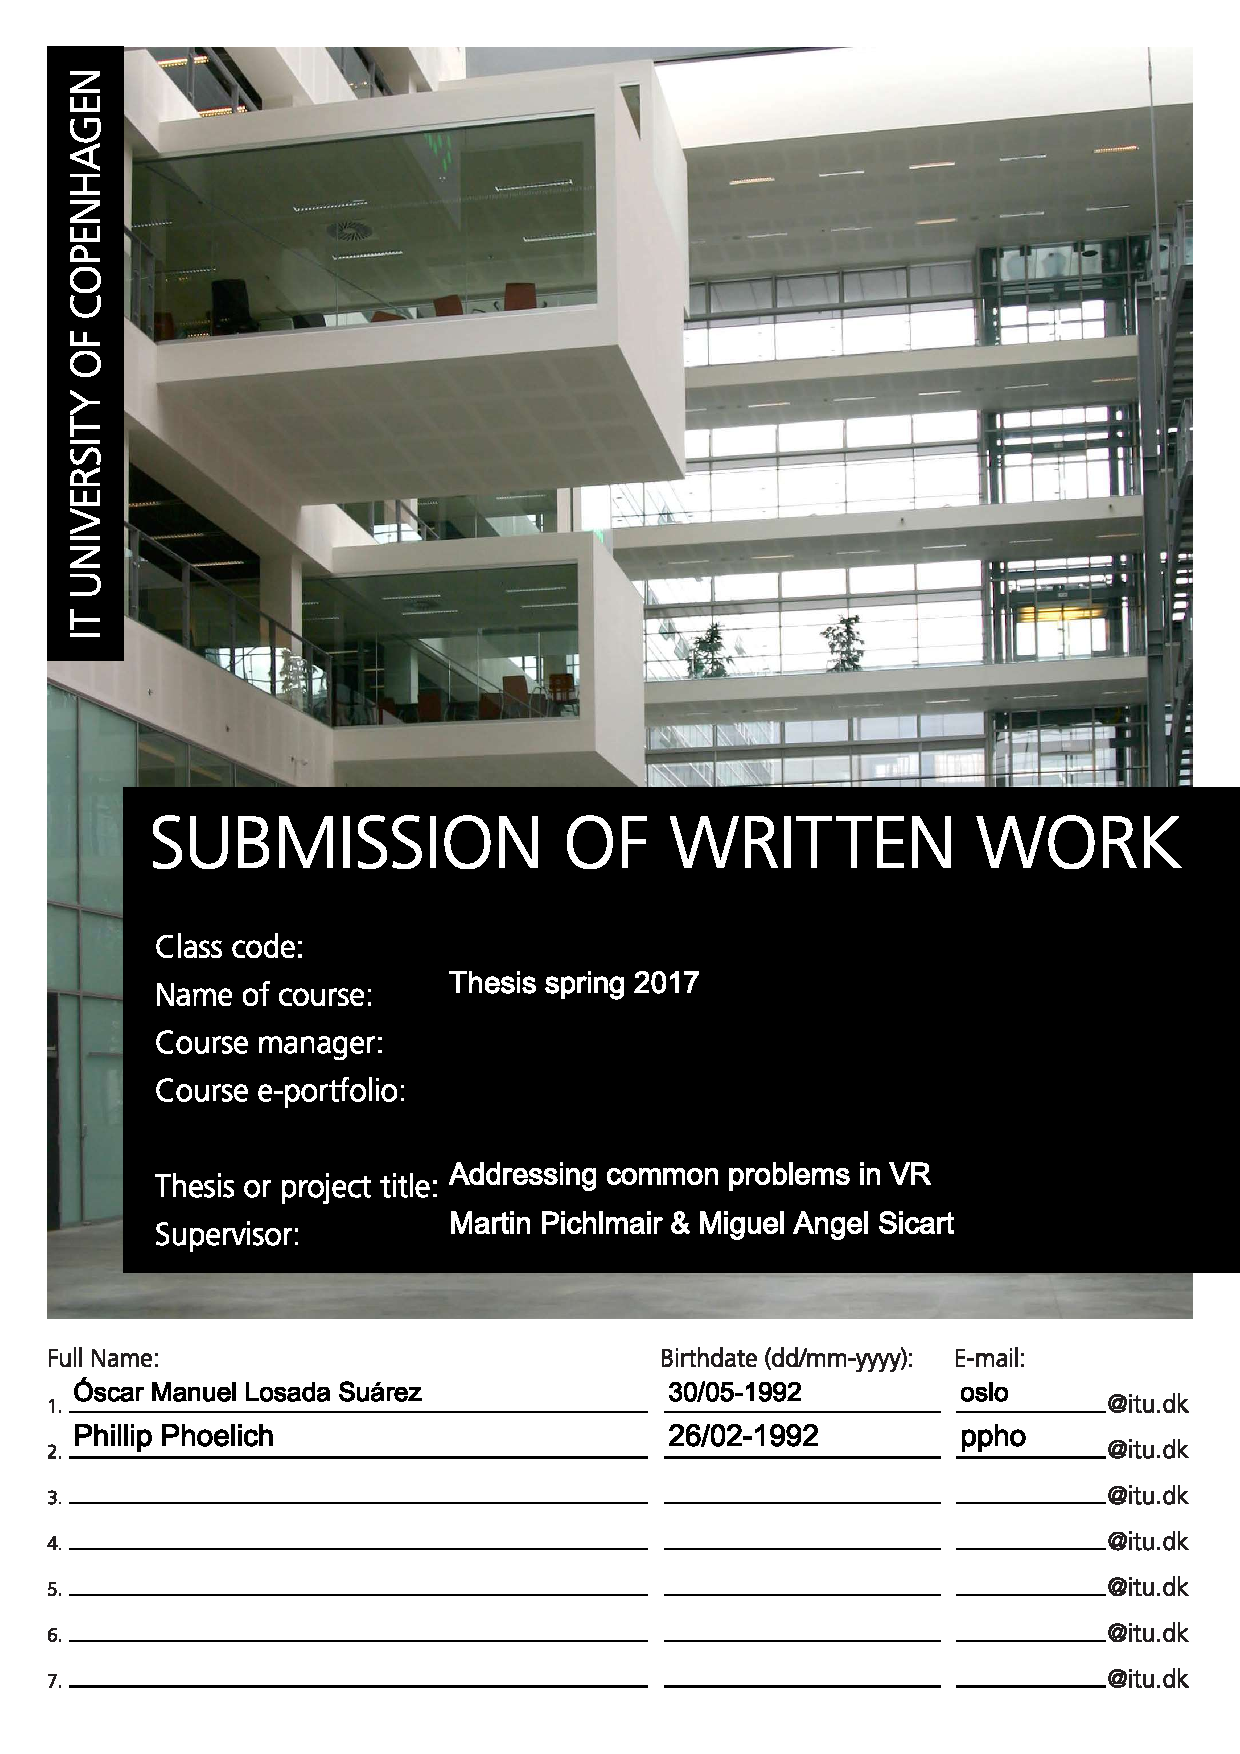
\includepdf{ITUfrontpage.pdf}

\listoftodos

% TITLEPAGE
\newgeometry{left=0.1cm,right=0.1cm}
\begin{titlepage}
\begin{center}

\textsc{\large Thesis paper}\\[2cm]

\textsc{\huge \textbf{Hands in Virtual Reality}}\\[8.2cm]
%\textsc{\large \textbf{With a focus on embodiement and the player's intensions}}\\[2cm]

\textit{Authors}\\
Óscar Manuel Losada Suárez\textit{(oslo@itu.dk)}\\
Phillip Phoelich \textit{(ppho@itu.dk)}\\[1cm]

\textit{Supervisors}\\
Martin Pichlmair\\
Miguel Sicart\\[1cm]

\textit{Date}\\
June 1st, 2017\\

\vfill
\textit{MSc in Games}\\
\textsc{IT University of Copenhagen}

\end{center}
\end{titlepage}

\restoregeometry

% ABSTRACT
\begin{abstract}
Here is the abstract of the thesis paper.
\end{abstract}

% TABLE OF CONTENTS
\tableofcontents
\newpage


%MAIN CONTENT
\newgeometry{top=3.9cm}

\chapter{Introduction}
\label{chap:introduction}
In our day-to-day lives, we constantly use our hands to hold, operate and otherwise manipulate objects, tools and devices with precision. We use them to gather tactile information about the world and even to communicate with each other through hand gestures and body language. They are a fundamental part of the human body and our way of interacting with the world around us.

The biggest buzzwords in the Virtual Reality (VR) medium: immersion and presence, perhaps point us in the right direction. VR is meant to bring us closer than ever before to experiencing virtual environments as if we were actually in them. Interaction is a big part of experiencing the places we are in. It should hardly be a point of contention then, that having virtual hands that imitate our own real hands can have a significant impact on VR experiences.

VR game developers and hardware manufactures alike have acknowledged this. Major consumer-oriented VR devices like the HTC Vive, the PlayStation VR  with the PlayStation Move Motion Controllers (PS VR + Move) and the Oculus Rift + Touch have controllers that track the position of your hands in space \parencite{htcvive2016, psvr2016, psmove2010, oculus2016}. In their About page, Owlchemy Labs, the creators of the critically and commercially acclaimed \parencite{UnityAwards2016, SteamSpyJobSim} Job Simulator: the 2050 archives \parencite{OwlchemyLabs2016} declare:

\begin{displayquote}
\textit{We believe that interaction and using your hands is what truly makes virtual reality the most incredible place to build unique content that blows players minds.} \parencite{aboutOwlchemyLabs}
\end{displayquote}

Predictably enough, this is not the end of the story. Even if we had complete tracking of the hands and individual fingers, the physical constraints of the virtual environment would still not apply to the users' real hands, which leaves us with few essentially different options:

\begin{enumerate}
\item Prioritize user input and ignore virtual environment constraints whenever there is a conflict in order to always keep the virtual hands aligned with the real hands to the extent allowed by the tracking data.
\item Separate the virtual hands from the real hands when there is conflict in order to respect the virtual environment's constraints.
\item Use sensory feedback that makes the users either respect the virtual constraints on their own or feel like they are constrained without actually being so.
\item As \parencite{Schell2015} suggests, design in a way that circumvents the problem, which means restricting the medium's content to experiences that fit exactly to the medium's current affordances \parencite{Norman}. This means seeing limitations as features and finding experiences that map perfectly to the current systems.
\end{enumerate}

The work here presented is focused on the second option, which is seen as a directly opposite alternative to the first. We aim to explore how virtual hands can work in this case and investigate whether the user experience can be improved with this approach.

From this point on, we will refer to this problem as the Virtual Constraints Problem, to the approaches fitting the first option as Unadjusted Hand Control Models and to those fitting the second option as Adjusted Hand Control Models.

\begin{figure}[h]
\centering
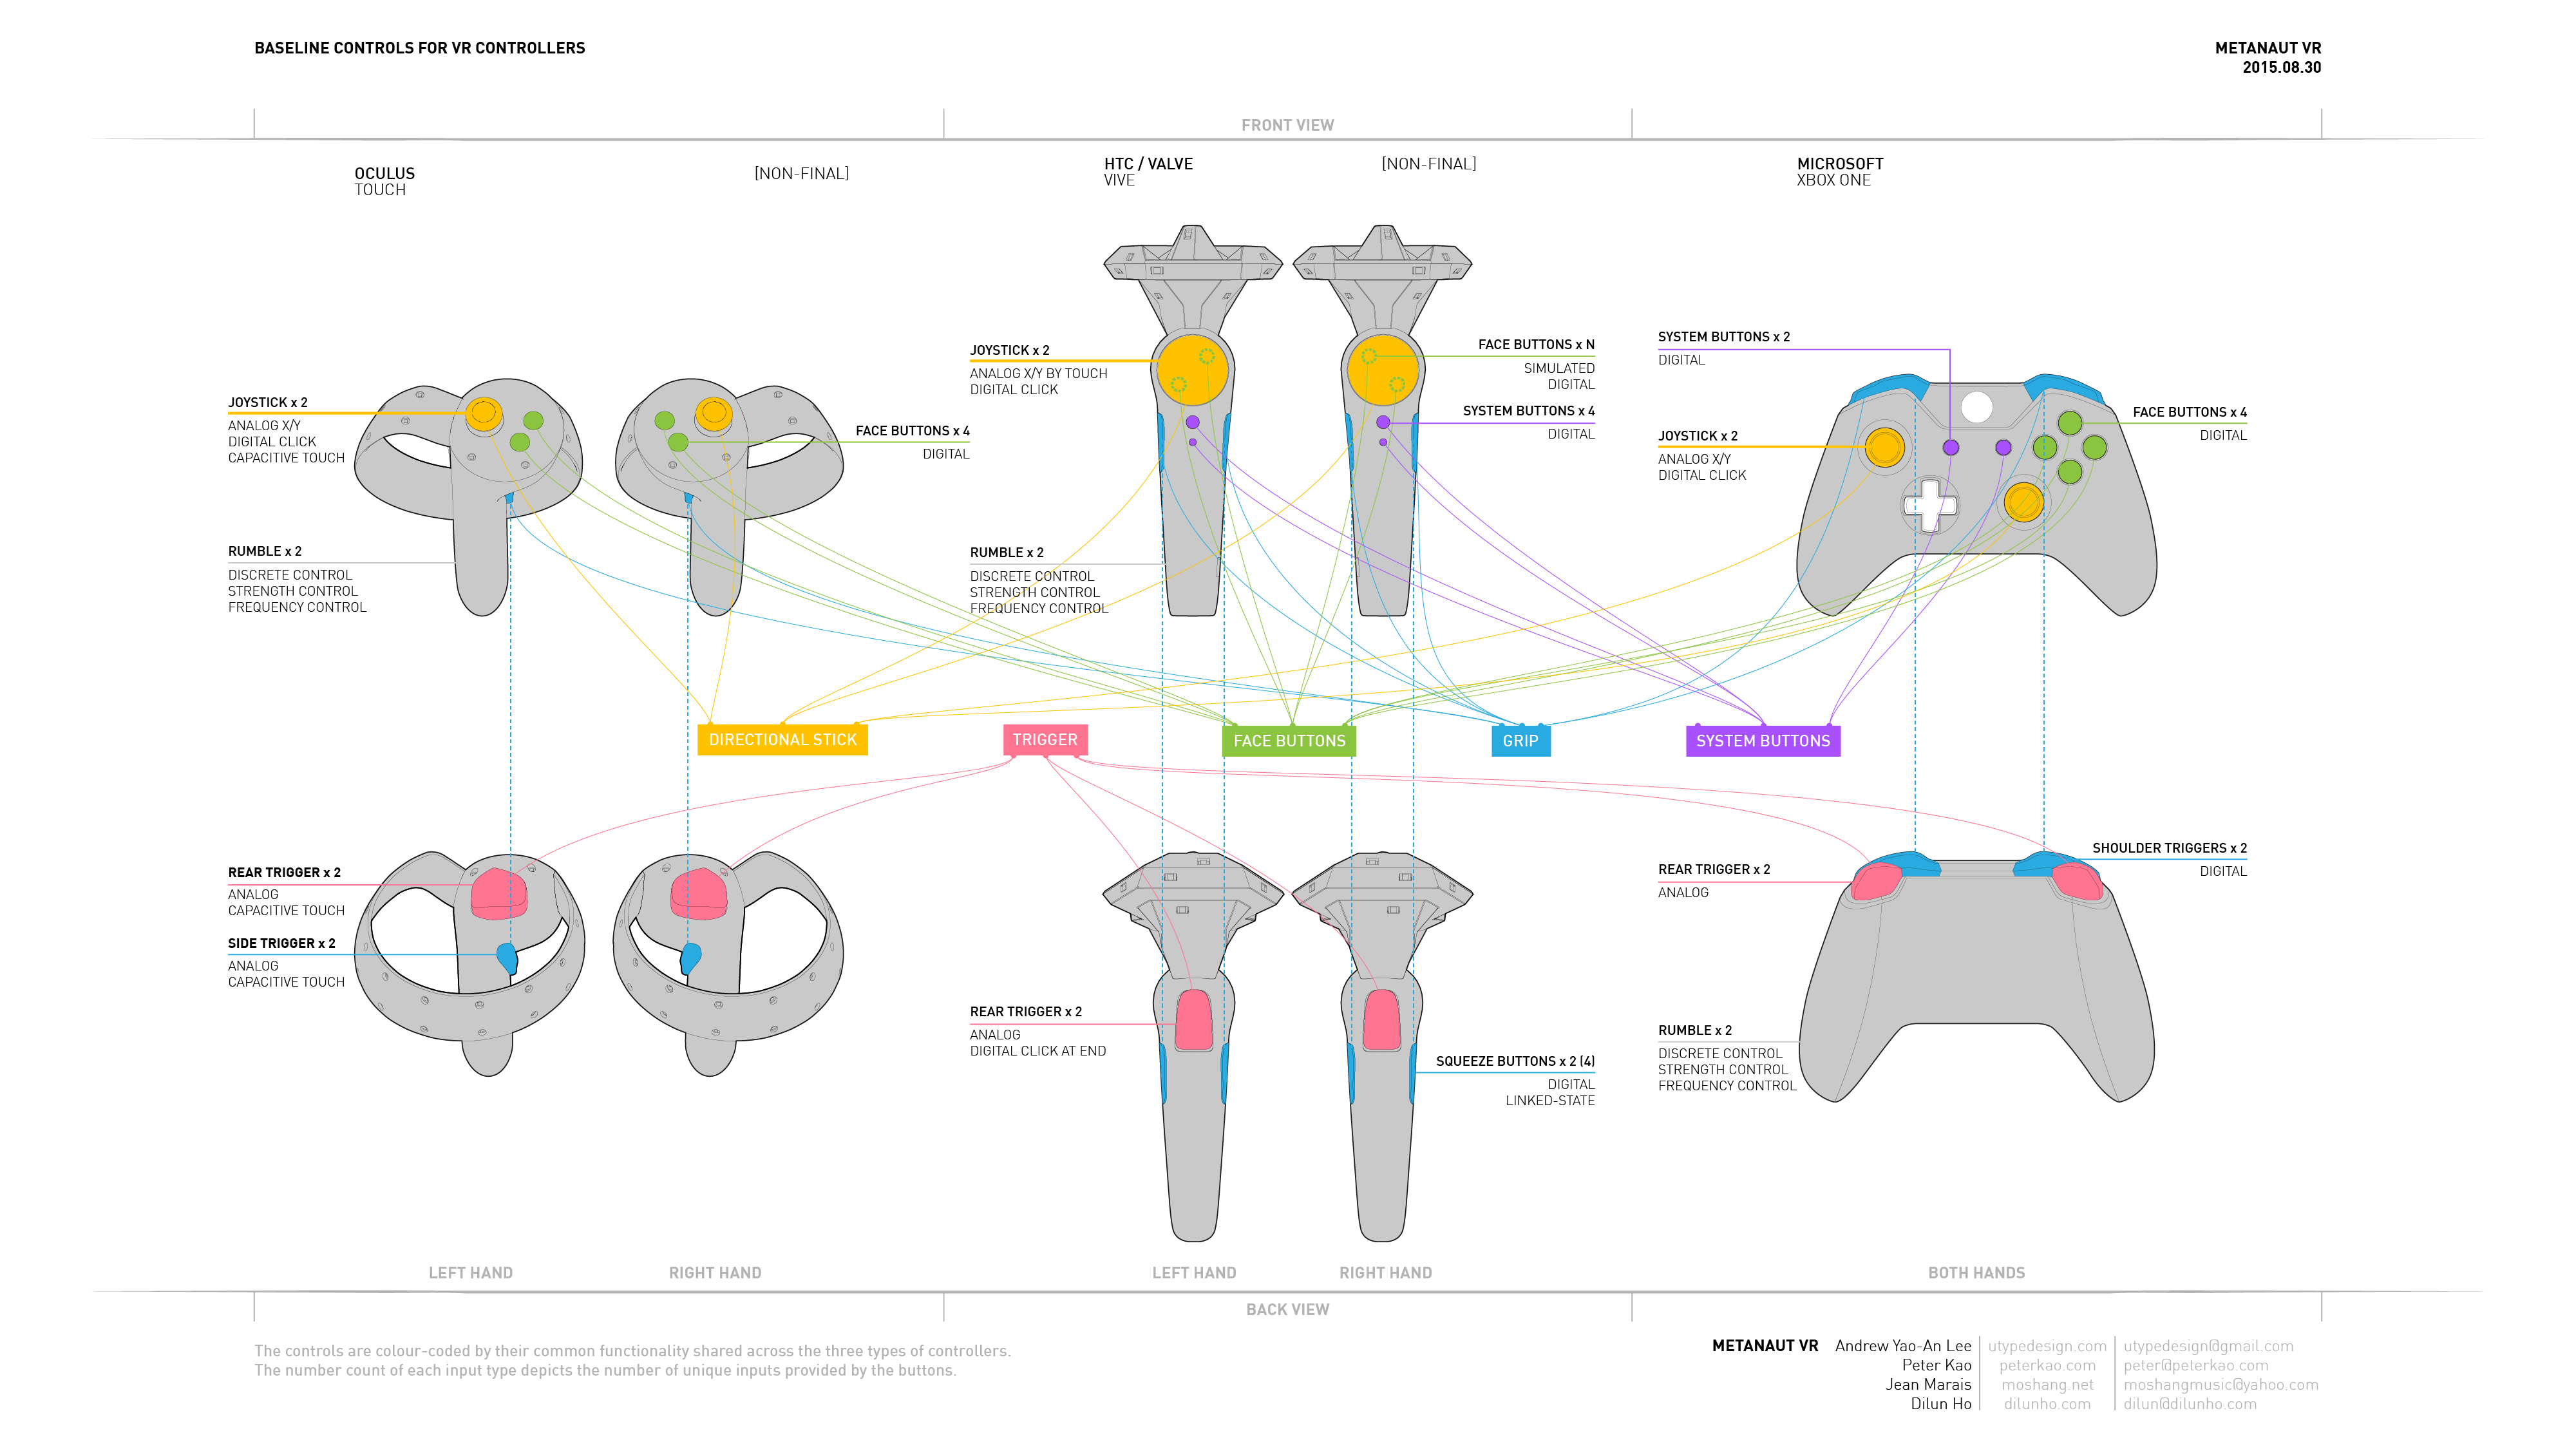
\includegraphics[width=\textwidth]{vrcontrollersbaselinecomparison2c.png}
\caption{Comparison of VR controllers and their different input and output capabilities. Note that the final version of the HTC Vive controllers looks different. Retrieved from\parencite{MetanautVR2015} and can be seen in a larger format in Appendix \ref{apx:vrControllerComparison}.}
\label{fig:vrControllerComparison}
\end{figure}

\section{State of the Art}
\label{sec:stateOfTheArt}

\subsection{VR Hardware}
\label{subsec:vrHardware}

There is a considerable amount of devices and accesories that are relevant to VR. This work is mainly applicable to those setups that can spatially track the hands of the user to a similar or greater degree than the HTC Vive allows. We are particularly interested in findings that are relevant to the aforementioned HTC Vive, PS VR + Move and the Oculus Rift + Touch because they are currently the most important consumer-oriented devices with these capabilities \parencite{Armstrong2017, SuperDataLLC2017}.



There are differences between the Head Mounted Displays (HMD) of these devices, but for the most part, they are not relevant for our area of focus, so they will not be discussed here.

On the other hand, it might be worth briefly covering the differences in terms of spacial tracking of the controllers between the devices. The HTC Vive allows 360 degree tracking within the biggest space volume, the Oculus Rift + Touch with the default setup is designed mainly for 180 degree tracking, but an experimental setup with extra components allows stable 360 tracking \parencite{Lang2016, Kuchera2016}.

Figure \ref{fig:vrControllerComparison} shows the features of the Oculus Touch and the HTC Vive controllers. In the case of the HTC Vive, the most relevant features for our purposes are:

\begin{itemize}
\item the analogue triggers with digital click at the end, controlled with the index finger, 
\item the digital grip buttons, pressed with middle, ring and/or pinky fingers,
\item the joysticks or trackpads, with analog x/y input through capacitive touch and digital click, used with the thumbs
\item and rumble capabilities.
\end{itemize}

In the case of the Oculus Touch, the relevant features are:

\begin{itemize}
\item the analogue triggers with capacitive touch, controlled with the index fingers, 
\item the analogue side triggers, pressed with middle, ring and/or pinky fingers,
\item the joysticks, with analog x/y input, digital click capacitive touch, used with the thumbs
\item and rumble capabilities.
\end{itemize}

Figure \ref{fig:psmoveDiagram} shows the input mechanisms of the PS Move Motion Controller, again, the most relevant features are:

\begin{itemize}
\item the analogue T buttons, controlled with the index fingers,
\item several digital buttons controlled by the thumbs
\item and rumble capabilities.
\end{itemize}

\begin{figure}[H]
\centering
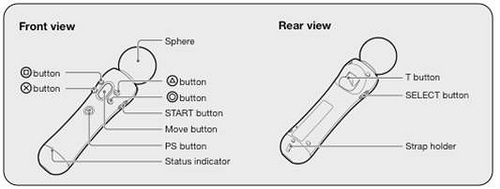
\includegraphics[width=\textwidth]{psmovecontroller.jpg}
\caption{Diagram of the PS Move Motion Controller. T button allows analogue input. Retrieved from \parencite{psmoveDiagram}.}
\label{fig:psmoveDiagram}
\end{figure}

Analogue buttons are useful to allow the users to control the motion of the virtual fingers with similar movements with their own fingers - in Norman's terms, they provide a natural mapping \parencite{Norman} for finger control. Similarly, although without the advantage of being analogue, buttons or areas with capacitive sensors can be used to monitor if the user's fingers are resting on the controller or are lifted, which can allow for guessing the position of the fingers. 

The Oculus Touch is the controller that takes these input mechanisms further having a capacitive trigger for the index finger, capacitive buttons for the thumb and a normal trigger for the other three fingers. This can be used to detect a variety of gestures like index finger pointing, thumbs up (or down), finger guns... It also facilitates common interactions like pressing virtual buttons with your virtual index finger, operating a grabbed object with the same hand that is holding it (e.g. press gun trigger). Both the HTC Vive and PS VR controllers allow for a lower degree of natural finger control.

Other accessories exist that allow for actual positional tracking of the fingers, such as the Manus VR Gloves \parencite{ManusVR2016}. These would of course enhance the experience, but ultimately would face the same problem because they don't provide a way to impose constraints from the virtual world on the real hands of the user.

\subsection{VR Games}
\label{subsec:vrGames}

The most frequent approach to dealing with the Virtual Constraints Problem described at the beginning of this chapter is to ignore these constraints when they conflict with the user input. Job Simulator is a prime example of the unadjusted hand model and the one that we have used in our work as a baseline for comparison.

In Job Simulator the hands never separate from the position of the controller, but this still allows for reasonable physical interaction with small, light objects that can be easily moved by the hands. When the hands collide with movable objects, the object is pushed out of the way. However, when the virtual hands collide with objects that cannot be moved by them, the hands will simply go through them as if they weren't there as shown in Figure \ref{fig:jobSimStaticProblem}.

\begin{figure}[H]
\centering
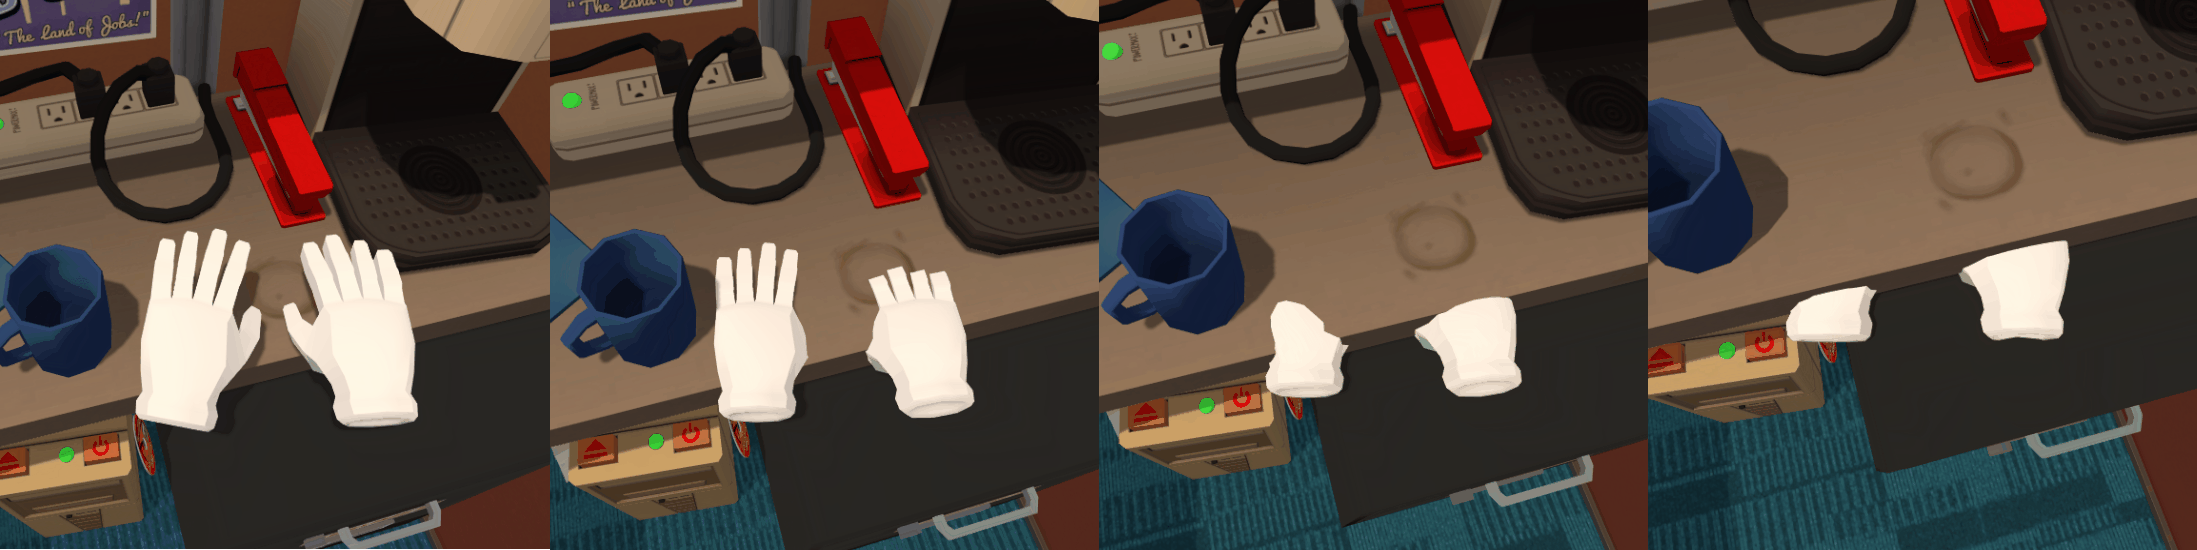
\includegraphics[width=\textwidth]{Sequences/JobSimulator/jomSimStaticProblem.png}
\caption{Sequence showing the Job Simulator hands entering an immovable obstacle. Captured in the HTC Vive version. A gif can be found here: \url{https://tinyurl.com/JobSimTouchStatic} .}
\label{fig:jobSimStaticProblem}
\end{figure}

At the same time, they avoid the problem of grabbing objects with correct finger placement by hiding the hands when they are holding an object as shown in Figure \ref{fig:jobSimGrabProblem}. This solution is not without merits: it allows the user to see the held object from all angles without the hand obstructing the view, it is simple and surprisingly, it is often not noticed by the users.

Ideally however, we would like the hand to be visible and the fingers to be correctly placed on the grabbed object forming a grip. But without adjusting the virtual hand, this requires the user to be too precise controlling the virtual hands and makes grabbing objects very difficult.

\begin{figure}[h]
\centering
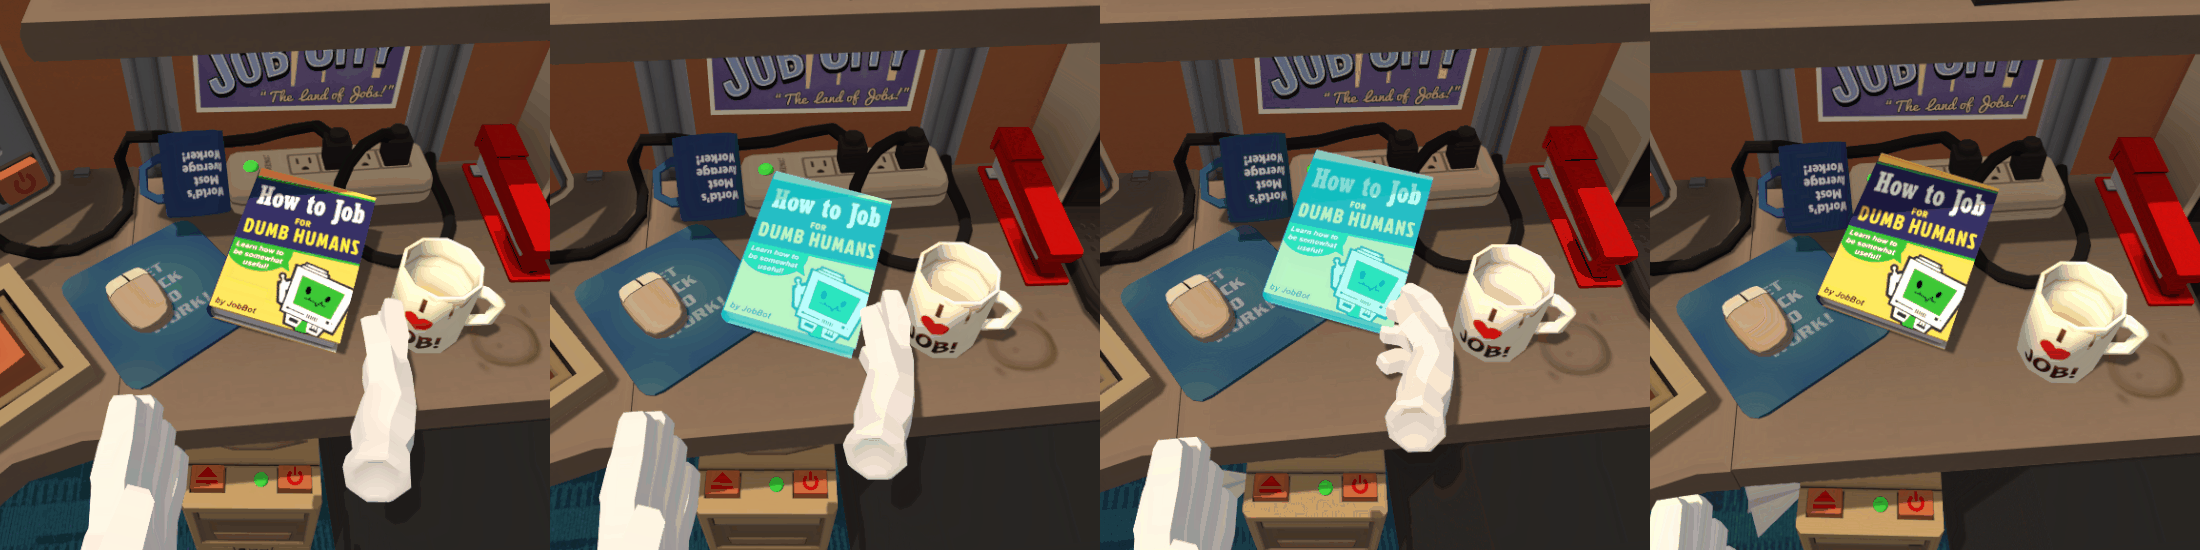
\includegraphics[width=\textwidth]{Sequences/JobSimulator/jomSimGrabProblem.png}
\caption{Sequence showing the Job Simulator hands grabbing an object. The hands are hidden while holding objects. Captured in the HTC Vive version. A gif can be found here: \url{https://tinyurl.com/JobSimGrabObject} .}
\label{fig:jobSimGrabProblem}
\end{figure}

Very recently, a few games have started to show approaches to hand control that fall within the adjusted hand model. One these is Wilson's Heart \parencite{TwistedPixelGames2017}, released in April this year. Each object that the user can interact with has a predefined hand pose and when certain conditions are met, the hands will snap to the pose as shown in Figure \ref{fig:wilsonGrab}. These conditions usually have to do with the user pressing some of the triggers or buttons that control the virtual fingers although there are also poses that are triggered by moving the hands close enough to the objects.

\begin{figure}[h]
\centering
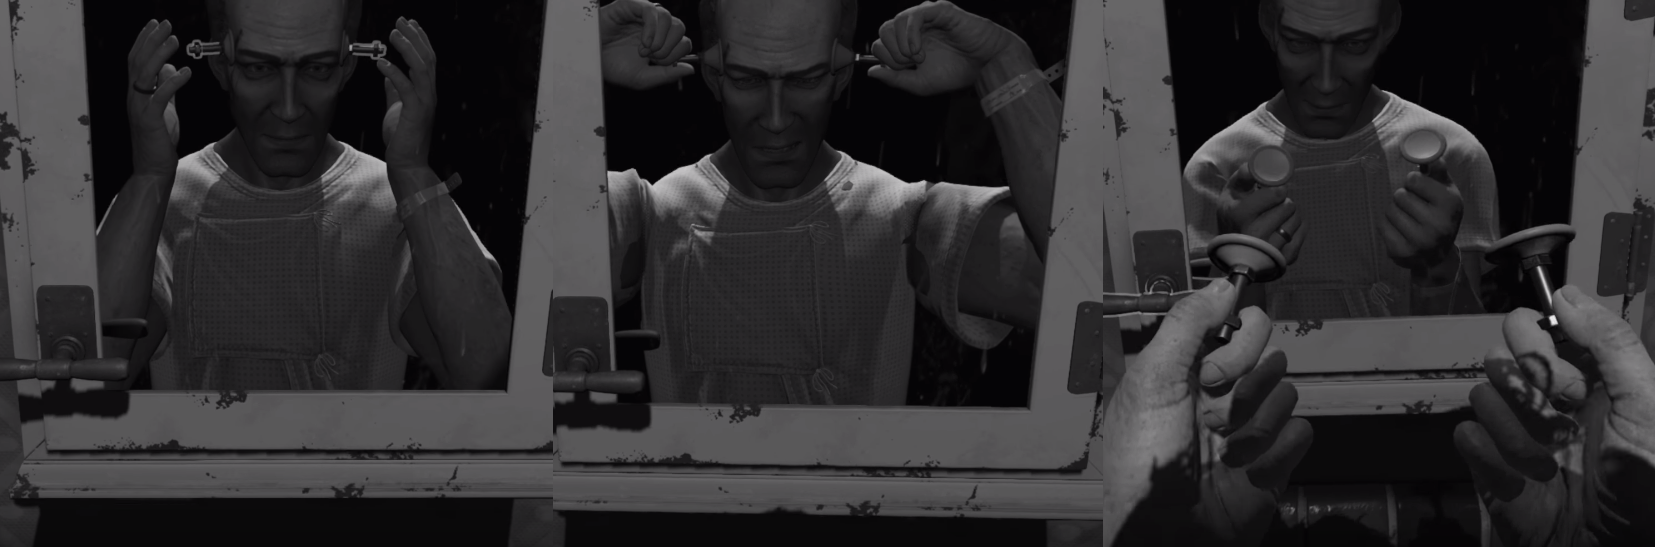
\includegraphics[width=\textwidth]{Sequences/WilsonsHeart/wilsonGrab.png}

\vspace{0.15cm}

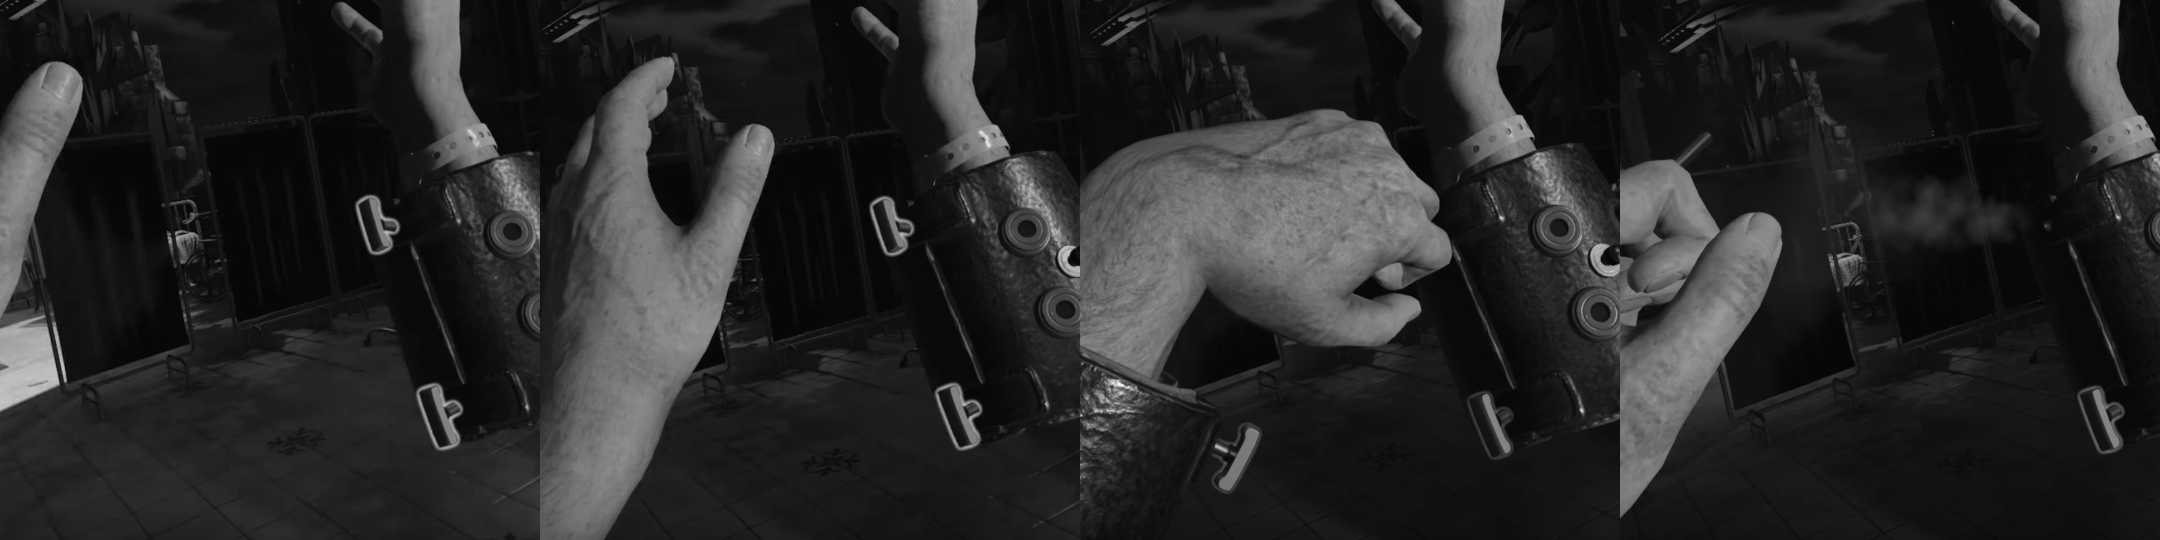
\includegraphics[width=\textwidth]{Sequences/WilsonsHeart/wilsonGrabCuffs.png}
\caption{Sequences showing the pose-snapping grab in Wilson's Heart. Two gifs showing the pose-snapping can be found here: \url{https://tinyurl.com/whGrabPoseMirror} and \url{https://tinyurl.com/whGrabPoseCuffs} .}
\label{fig:wilsonGrab}
\end{figure}

This technique is interesting because the virtual hands can separate a lot from the position of the real hands and very suddenly too. The underlying idea is that user's want to interact with each object in a certain way and will on their own pose their hands in a similar way to the object's pose, so when the pose snapping happens, the change will be small and, most importantly, aligned with the user's intention. 

The pose-snapping method allows perfect placement of the fingers and looks great in pictures, but it requires a lot of manual work to setup every interactible object in the game and it takes away a lot of control from the users, forcing them to interact with each object exactly in the ways that the poses allow.

\begin{figure}[h]
\centering
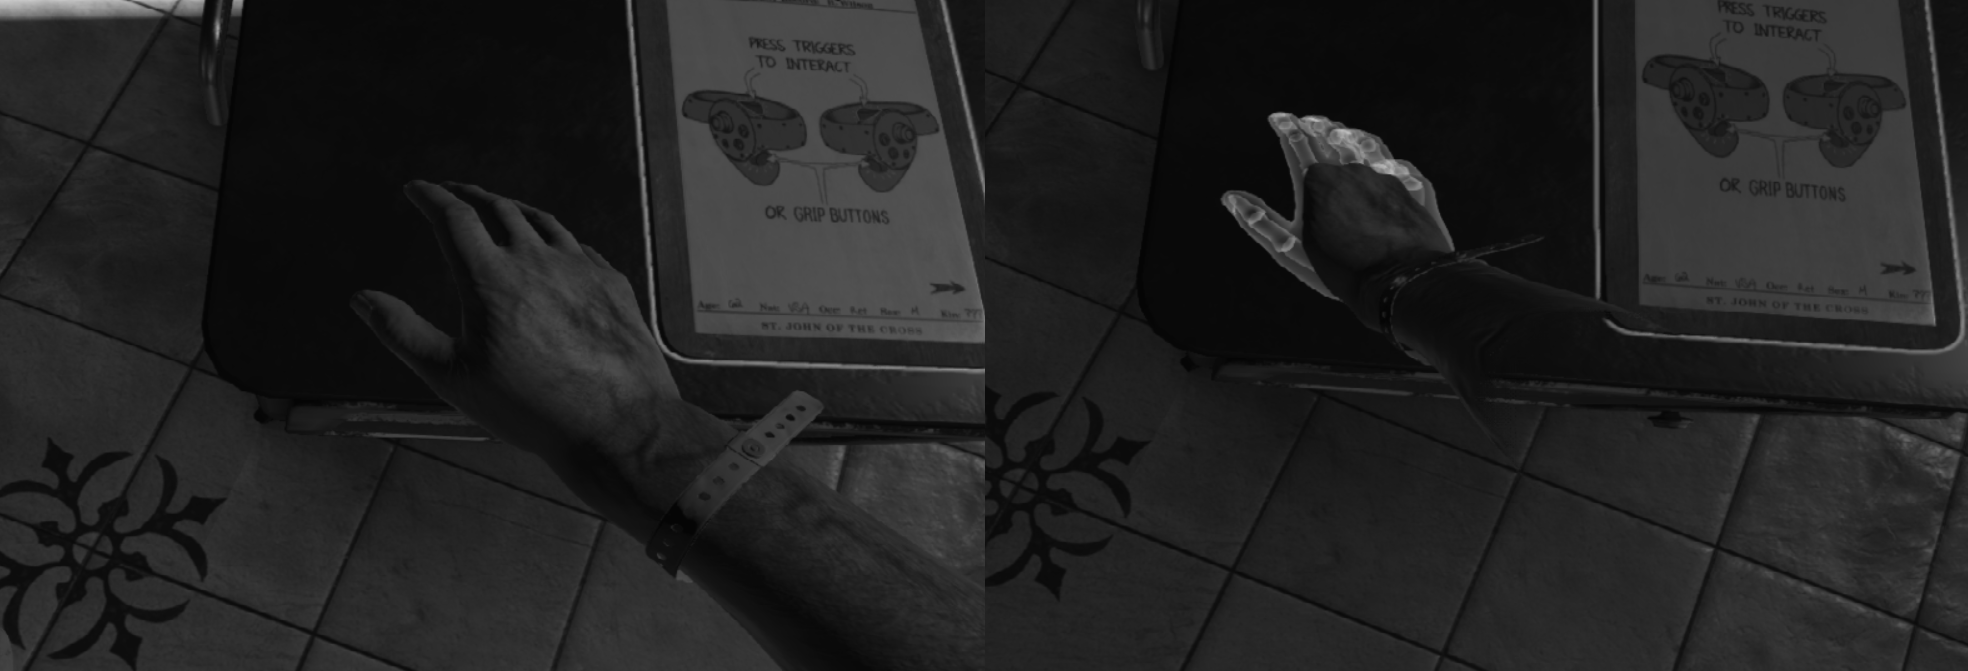
\includegraphics[width=\textwidth]{Sequences/WilsonsHeart/wilsonPenetration.png}
\caption{Sequence showing the hands in Wilson's Heart entering an immovable object. An X-Ray effect shows the part of the hand inside the object. A gif can be found here: \url{https://tinyurl.com/whPenetration} .}
\label{fig:wilsonPenetration}
\end{figure}

Figure \ref{fig:wilsonPenetration} shows that the other issue identified with the Job Simulator hands is mostly unsolved in Wilson's Heart. The hands can still go through immovable objects, but in this case, an X-Ray style effect is used to visualize the parts of the hands that are inside of objects. This communicates the state of the hands to the player, but might not be preferable to other techniques that make the virtual hands respect the virtual world's physics.

The most novel and promising attempt within the adjusted hand model that we are aware of however, is an upcoming game called Lone Echo \parencite{ReadyAtDawn}. In this game, the virtual hands procedurally adapt to the virtual environment. Once again, the underlying principle is adjusting the virtual hand in a way that doesn't conflict with the user's intentions, but in this case instead of using authored poses the use of a real-time algorithm can make the system extremely flexible. At its best, this approach could empower the user and make them feel more control over their virtual hands by not forcing the interaction with objects to one specific pose. At its worse, there might be situations where the algorithm doesn't behave in a way that matches the user's natural way of interacting with their hands which would have the opposite effect.

This approach will inevitably come at the cost of having some edge cases that don't look as good authored poses, but in terms of development work, scales much better with the amount of objects in the virtual environment and these edge cases might be so rare that they barely impact the experience.

Figure \ref{fig:loneEchoGrip} tries to show the procedural hand posing shown in some of the available footage from the game, but in this case particularly - and in general for the other frame sequences included in this work - we encourage the reader to watch the linked videos and .gifs because a few frames can't possibly do them justice.

\begin{figure}[H]
\centering
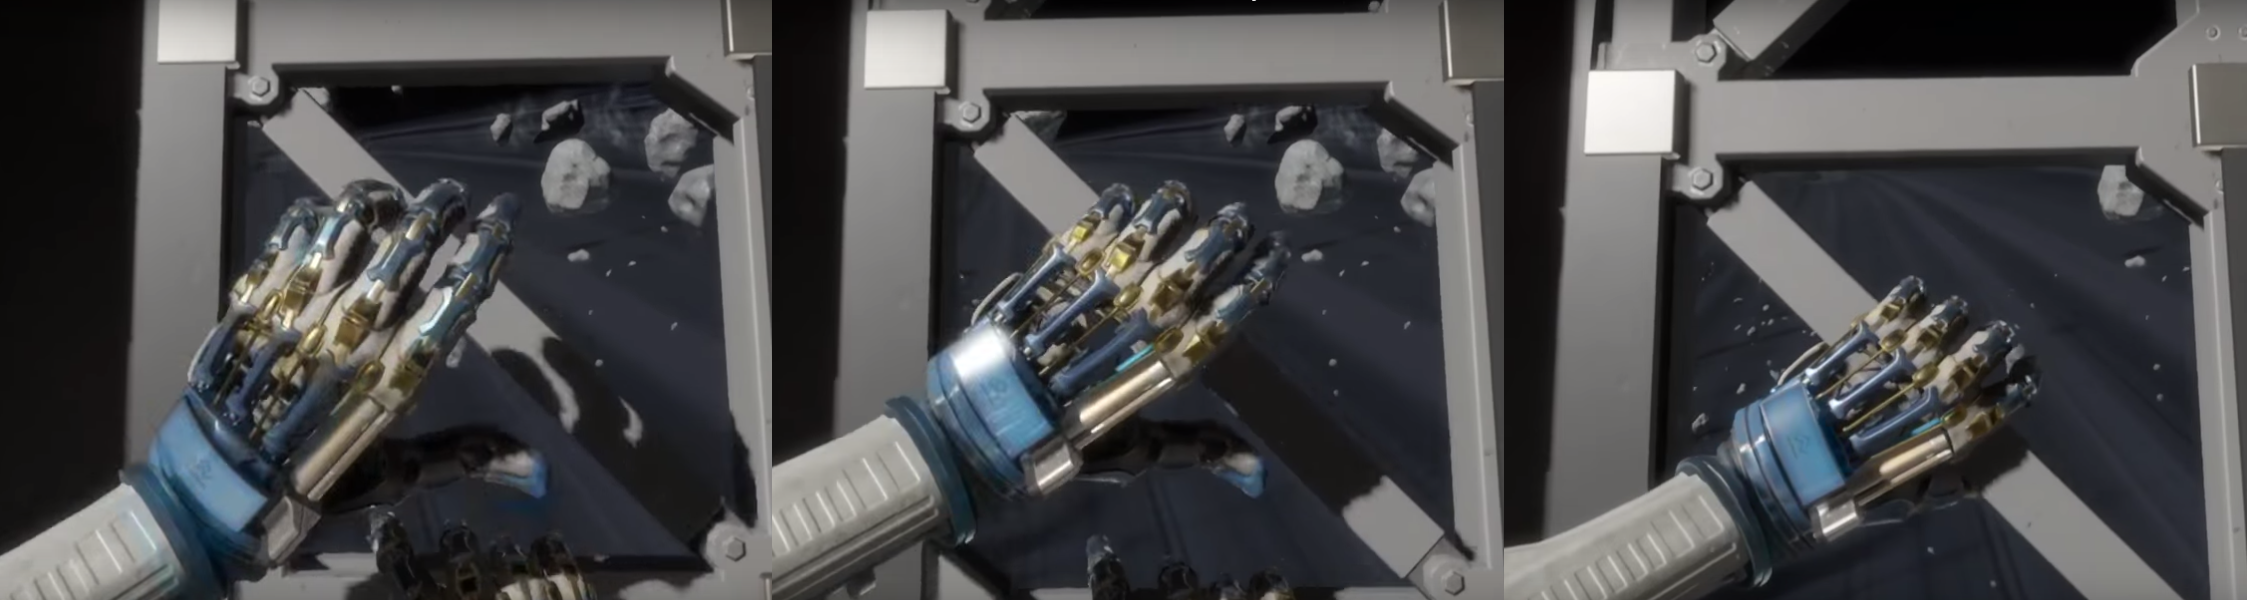
\includegraphics[width=\textwidth]{Sequences/LoneEcho/loneEchoGrip.png}
\caption{Sequence showing the procedural hand posing system in Lone Echo. Captured from video \parencite{loneEchoVideo}. The video can be found here: \url{https://tinyurl.com/loneEchoVideo} .}
\label{fig:loneEchoGrip}
\end{figure}

\section{Research Questions}
\label{sec:researchQuestions}

This work explores ways of dealing with the Virtual Constraints Problem previously described: how can we deal with the conflict between wanting the virtual hands to imitate the user's real hands and at the same time respect the virtual environment?

We consider this problem to be specially prominent in two use cases:

\begin{enumerate}
\item The user places his real hand in a way that would make the corresponding virtual hand be inside of another virtual solid object.
\item The user wants to grab a virtual object but doesn't position the controller and otherwise produce the input that would in a strict simulation allow their virtual hand to lift the object.
\end{enumerate}

These properties should be pursued without losing the degree of control, consistency and intuitiveness that existing unadjusted hand models provide. In sum, the degree of "hand presence" (term commonly used in the VR industry \parencite{Bye2016}) achieved by this model cannot be lost in favor of these goals. The question this work addresses is whether "hand presence" can be improved by dealing with the virtual environment constraints problem.

As secondary objectives, we are interested in finding ways of conveying a sense of the weight of virtual objects when interacting with them and improving the tactility of the virtual hands, improving the feeling of touching virtual objects, which are also aspects currently unsatisfactorily addressed.

Therefore, we are trying to reduce the existing gap between the user's real body and their virtual body and compensate for imprecise user input. In terms of the user's perceptual, sensory experience, it might be possible to improve how hands are controlled in VR.

We focus on experimenting with different ways of adjusting the virtual hands' pose, exploring possible adjusted hand models. We will use the Job Simulator hand model, a great example of an unadjusted hand model, as a reference and baseline to compare our experiments with.

\restoregeometry
\newpage

\chapter{Methodology}
\label{chap:methodology}

\restoregeometry
\newpage

\chapter{State of the art}
\label{chap:stateOfTheArt}

\restoregeometry
\newpage

\chapter{Implementation}
\label{chap:implementation}
\begin{itemize}
\item Introduction for the implementation section.
\item Introduction should perhaps introduce the topics of this chapter.
\end{itemize}

\textbf{What is the implementation chapter about?}\\
This chapter delves into the development of several prototypes, each portraying different types of behaviour for hands in VR. These different prototypes have similarities and differences in their approach to the problem. In the following sections we will present a categorization of approaches that can be taken when implementing hands in VR, what effect these different approaches have and their pros and cons.

\textbf{What stuff did we use during the project?} (headset and control scheme, for instance)\\
The prototypes have all been developed using the Unity engine which means that to their implementations are restricted by the API that Unity provides. Furthermore, during development and testing, we’ve been using the HTC Vive and its default controllers as the input method for the hands.

Since we have been using the HTC Vive and its default controllers as input to control the hands our approaches are more applicable to hardware that has the same affordances as these controllers. We use the position and orientation input from the controllers to position and rotate the hands in the virtual space and we use the trigger button to indicate how much the fingers should bend or how closed the hand should be.

\todo[inline]{Mention the use of Unity as well.}

\textbf{How does this lead into the categorizations?}\\
These three inputs are the base of the categorizations of approaches. Each of these inputs can be filtered, by which is meant that the input can be modified or skipped. Filtering on one of the inputs can be seen as using that input as the parameter for a function, which returns a new result. A hand can have a filter for either none of the inputs or one of the inputs or more. Different filtering combinations will give a different behaviour for the hand in the virtual world and might result in the hand seeming more realistic when interacting with its environment.

\section{Categorization of approaches}
\label{sec:categorizationOfApproaches}
\begin{itemize}
\item Lead into the explanation for the filter variables.
\item Display filter variable table.
\item Describe several examples of filter variable combinations and show image sequences.
\item (Describe the reasons and effects for filtering on the different variables)?
\end{itemize}

The three player inputs mentioned above (position, orientation and how closed the hand should be) are the base of the categorization of approaches. Each of these inputs can be filtered, by which is meant that the input can be modified or skipped. Filtering on one of the inputs can be seen as using the input as the parameter for a function, which returns a new result which will be used instead of that input. A hand can be implemented with filters on several inputs at once and can have different filters depending on the context. Different filterer combinations will give a different behaviour for the hand in the virtual world and can result in the hand seeming more realistic when interacting with its environment.

\begin{table}[H]
\centering
\caption{Filter variable combinations.}
\label{tab:filterVariableCombinations}
\begin{tabular}{C{2cm}C{2cm}C{2cm}}
Position & Rotation & Finger position \\ \midrule \midrule
         &          &                 \\ \midrule
\Large X &          &                 \\ \midrule
         & \Large X &                 \\ \midrule
         &          & \Large X        \\ \midrule
\Large X & \Large X &                 \\ \midrule
\Large X &          & \Large X        \\ \midrule
         & \Large X & \Large X        \\ \midrule
\Large X & \Large X & \Large X       
\end{tabular}
\end{table}

\subsection{Position filtering}
\label{subsec:categoryPositionFiltering}
\textbf{Questions to answer in this section:}
\begin{itemize}
\item What does it mean to filter the player's positional input?
\item Why do we want to filter the player's positional input?
\end{itemize}

\textbf{What does it mean to filter the player's positional input?}\\
A position filter using the definition above is a function, which when enabled, takes the player's positional input from a controller and returns a new value to be used in its stead. This means that the position of the hand in the virtual world will deviate from the controller position.

\textbf{Why do we want to filter the player's positional input?}\\
One of our hypotheses is that it's possible to increase the player's sense of embodiment by simulating more realistic behaviour for hands around objects in the world. One of the first steps here is to not allow the hands to penetrate objects. By using position filtering to deviate the hand from the controller position when trying to penetrate an object, the hand can interact more realistically with the world.

The following two figures show an image sequence of a hand with no input filtering and an image sequence with a hand that uses position filtering. The second figure shows that the hand is stopping when it reaches the object, whereas in the first figure the hand moves through the object.

\begin{figure}[H]
\label{fig:filtersNone}
\centering
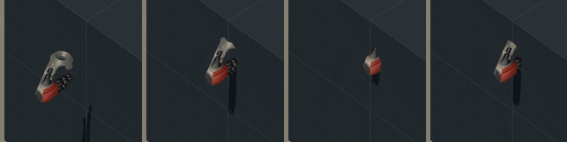
\includegraphics[width=\textwidth]{Sequences/FiltersNone/Seq_FiltersNone.png}
\caption{Sequence showing hand without filters entering obstacle.}
\end{figure}

\begin{figure}[H]
\label{fig:filtersPosition}
\centering
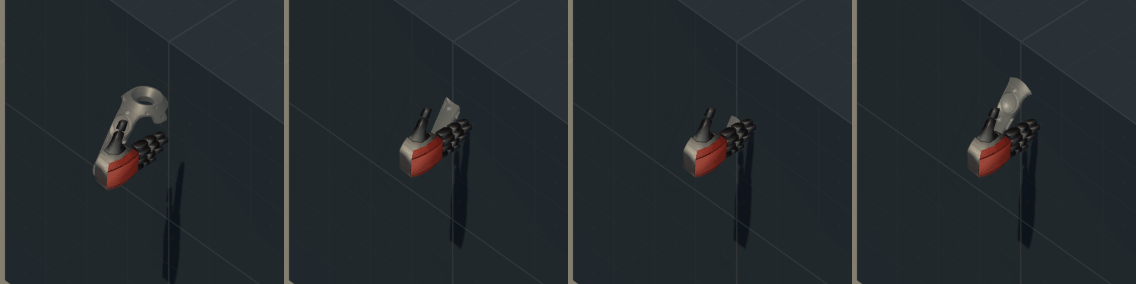
\includegraphics[width=\textwidth]{Sequences/FiltersPosition/Seq_FiltersPosition.png}
\caption{Sequence showing hand filtering on position. Notice the controller continuing to move into the obstacle.}
\end{figure}

\textbf{Questions to answer in this section:}
\begin{itemize}
\item How can we filter the player's positional input?
\begin{itemize}
\item Depenetration.
\item Physics system.
\item Different filter methods have different restrictions.
\end{itemize}
\end{itemize}

\textbf{How can we filter the player's positional input?}\\
The position filters we have implemented can be split into two distinct categories: a pre-collision correction category and a post-collision correction category. Using a pre-collision correction method in the case of disallowing the penetration of objects means to never allow the hand to enter an object by anticipating the penetration in advance. Using a post-collision correction method in the same case means to correct the hand's position after the collision has happened.





Position filtering in the case of disallowing the penetration of objects can be implemented in several ways. One of the methods used during this thesis project is to detect a collision between the hand and an object in the world and take action when such a collision occurs. The manual collision checking can be implemented by checking for nearby object colliders and using ray casts or sweeps to anticipate the collision.

Another implementation uses the physics system to handle collisions between the hands and obstacles in the world. The hands are moved by setting their velocities in such a way that they would reach their target within the current frame.

\subsection{Rotation filtering}
\label{subsec:categoryRotationFiltering}
\textbf{Questions to answer in this section:}
\todo{Alternative term: orientation}
\begin{itemize}
\item What does it mean to filter the player's rotational input?
\item Why do we want to filter the player's rotational input?
\begin{itemize}
\item Reduce position filtering.
\item Display player's intentions.
\item Diagetically communicate available interactions.
\item Allows for more detailed hand animation depending on available interactions. Control?
\item Mention stiffness with only position filtering
\end{itemize}
\end{itemize}

\textbf{What does it mean to filter the player's rotational input?}\\
To use a rotation filter is to deviate the hands rotation from the current orientation of the controller. In certain contexts it can be beneficial filter on rotation on order for the hand to seem more alive and realistic. Hands can adapt their rotation in several ways and different approaches might be taken depending on the context. When approaching a wall with their hand a player's intention in the real world might be to place their hand flat on the wall (palm-first). This behaviour can be implemented using a rotation filter, which takes effect when the hand is approaching a surface.


\todo[inline]{Adjusting might be a better word?} Filtering on the rotation input means to rotate the hand differently in the virtual world compared to the rotation of the controller.

\textbf{Why do we want to filter the player's rotational input?}\\
Rotation filtering can be used to display what is assumed to be the player's intention when they interact with the world. One example could be the intention of the player when they approach a wall with their hand. In this case a reasonable assumption would be that the player's intention is to rotate the hand so that the palm faces the wall (See image sequences below). Besides being useful when wanting to adapt the hand to the player's intentions, rotation filtering can also be used in order to reduce the amount of position filtering needed. This means that rotating the hand will allow the distance between the hand and the controller due to position adjusting to be reduced (See image sequence below).

\todo[inline]{use refs}
The first of the two figures below shows an image sequence of a hand using only rotation filtering and the second figure shows an image sequence of a hand using both position and rotation filtering where the rotation filtering is implemented as palm-first towards the surface.

\missingfigure[figwidth=15cm]{Image sequence: Rotation filtering}
\missingfigure[figwidth=15cm]{Image sequence: Position and rotation filtering}

\textbf{Questions to answer in this section:}
\begin{itemize}
\item How can we filter the player's rotational input?
\begin{itemize}
\item Manual rotation filtering when approaching obstacles.
\item Differentiation between object types and angles of approach.
\item Physics system.
\end{itemize}
\end{itemize}

\textbf{How can we filter the player's rotational input?}\\
Compared to position filtering, the way to implement rotation filtering is very much influenced by the assumptions about the player's intentions. When a player approaches a wall with their hand one assumption could be that the player's intention is to let their hand face the wall palm-first. This would manifest itself as a form of rotation filtering where the hand will rotate when nearing walls. While a player might want to approach a wall palm-first, their intentions might be different when approaching other types of objects like certain smaller grabbable objects which could have a specific pose for the hand to rotate towards. Another parameter which might help decide how to adapt the rotation is the angle of approach. When approaching a surface the rotation target might differ depending on if it's the front or the back of the hand that is facing the surface.

\todo{"pressed firmly"?}
Another approach entirely is to let the physics system handle rotation filtering. This at first will not make a difference when the hand is touching an object, but when pressed firmly against a surface the hand will rotate as to reduce the distance between itself and the controller position.

\subsection{Finger position filtering}
\label{subsec:categoryFingerFiltering}
\textbf{Questions to answer in this section:}
\begin{itemize}
\item What does it mean to filter the player's finger position input?
\item Why do we want to filter the player's finger position input?
\begin{itemize}
\item Reduce position filtering.
\item Display player's intention.
\end{itemize}
\end{itemize}

\textbf{What does it mean to filter the player's finger position input?}\\
Filtering the finger positions is about placing the finger tips in space relatively to the rest of the hand or put differently; stretching and bending the fingers. The fingers can be filtered as a group or individually and different contexts can determine different filters.

\textbf{Why do we want to filter the player's finger position input?}\\
Here, like with the rotation filtering, a certain amount of assumptions have to be made about what the player's intend is. When a player's hand is approaching an object that can be grabbed, the most common case might be that they are trying to grab the object. If this is the case, adjusting the fingers to form a grip could be a natural behaviour.

\missingfigure[figwidth=15cm]{Image sequence: Position and finger position filtering}

\textbf{Questions to answer in this section:}
\begin{itemize}
\item How can we filter the player's finger position input?
\begin{itemize}
\item Filtering to avoid obstacles.
\item Filtering to anticipate player intent.
\item Differentiation between object types and angles of approach.
\end{itemize}
\end{itemize}

\textbf{How can we filter the player's finger position input?}\\
Implementations of finger position filtering include using an animation system to animate the fingers together or individually to different poses and the use of an Inverse Kinematics (IK) system to infer finger pose from finger tip position and hand position and orientation.

\todo{Obviously you skipped the actual methods?}

\section{Description of how we evaluated hand iterations ...}
\label{sec:DESCRIPTIONOFEVALUATIONSCENARIOS}
\todo[inline]{should this be methodology?}

\section{Hands and their filterings}
\label{sec:LABELABOUTHANDSVERSIONS}
\begin{itemize}
\item Describe each hand and what filtering variables they use.
\item Relate hands to the above filtering variable descriptions.
\end{itemize}

\section{Miscellaneous shitz}
\label{sec:MISCELLANEOUSSHITZ}

\subsection{Hand visualization}
\label{subsec:handVisualization}

\subsection{Rumblez!}
\label{subsec:RUMLBEZ}

\subsection{Grabbing system details}
\label{subsec:grabbingSystem}

\restoregeometry
\newpage

\chapter{Experiments and results}
\label{chap:experiments}

\restoregeometry
\newpage

\chapter{Conclusion}
\label{chap:conclusion}

%\input{somepage.tex}

%\bibliography{bibliography.bib}
\printbibliography

\end{document}